\chapter{Methodology}
\section{Overview of the Proposed System}


This project introduces \textbf{MStacking}, a novel heterogeneous federated learning (FL) framework for classifying abnormal heart sounds from decentralized, privacy-sensitive data. The key challenge addressed is that hospitals often use different machine learning models suited to their data and computing capabilities, and typically only have access to a subset of heart sound classes—leading to label misalignment.

To solve this, MStacking employs a stacking ensemble strategy. Each hospital (client) trains a binary classifier using its local data—usually covering one abnormal class and the normal class—and sends prediction scores and density estimations (not raw data) to a central server. There, a meta-learner integrates these diverse outputs into a unified, global multi-class model, enabling collaborative learning without compromising patient privacy.

A summary of prominent studies utilizing the PhysioNet/CinC 2016 dataset is presented in Table~\ref{tab:physionet_summary}, highlighting the evolution of machine learning applications in heart sound classification.

\begin{table}[h]
\centering
\caption{Summary of Studies Using the PhysioNet/CinC Challenge 2016}
\label{tab:physionet_summary}
\begin{tabular}{|p{3.5cm}|p{1.5cm}|p{3.5cm}|p{3cm}|p{4cm}|}
\hline
\textbf{Study} & \textbf{Year} & \textbf{Task} & \textbf{Model(s) Used} & \textbf{Contribution} \\
\hline
\cite{clifford2016classification} & 2016 & Normal/Abnormal Classification & Ensemble SVMs & Introduced the PhysioNet Challenge dataset \\
\hline
\cite{liu2016open} & 2016 & Classifier Evaluation & Open baseline models & Created open-access benchmark for PCG classifiers \\
\hline
\cite{wang2023explainability} & 2023 & Explainability in PCG Detection & SHAP + FNN & Applied feature attribution methods to enhance transparency \\
\hline
\cite{qiu2022fl} & 2022 & FL for Binary Heart Sound Detection & CNN (FedAvg) & Early federated prototype for heart sound classification \\
\hline
Qiu et al. (This Work) & 2024 & Multi-Class FL for PCG Analysis & RF, FNN, CNN (Hetero) & Introduces MStacking with misaligned labels and heterogeneity \\
\hline
\end{tabular}
\end{table}

\section{Local Model Architecture}

\subsection{Local Model Architecture}
\label{sec:local_model_architecture}

In the MStacking setup, each hospital independently chooses and trains a binary classifier tailored to its dataset size, signal type, and computational capacity (see Figure~\ref{fig:local_models}). Three model types are supported:

\begin{itemize}
    \item \textbf{Random Forest (RF)}: Ideal for low-resource clients with structured feature data. RF ensembles decision trees built on bootstrap samples and uses the Gini index for splits.
    
    \item \textbf{Feedforward Neural Network (FNN)}: Suitable for clients with moderate resources and low-dimensional data. FNNs learn non-linear patterns through layers of neurons trained via backpropagation.
    
    \item \textbf{Convolutional Neural Network (CNN)}: Best for institutions handling spectrograms (e.g., from Continuous Wavelet Transform). CNNs use convolutional layers, global adaptive pooling (GAP), and fully connected layers to classify input efficiently.
\end{itemize}

All models are trained using cross-entropy loss and the Adam optimizer. Clients follow a ``star-structured'' label setup—each has the normal class ($y=0$) and one abnormal class ($y=m$), mimicking real-world healthcare data limitations.

\begin{figure}[h]
    \centering
    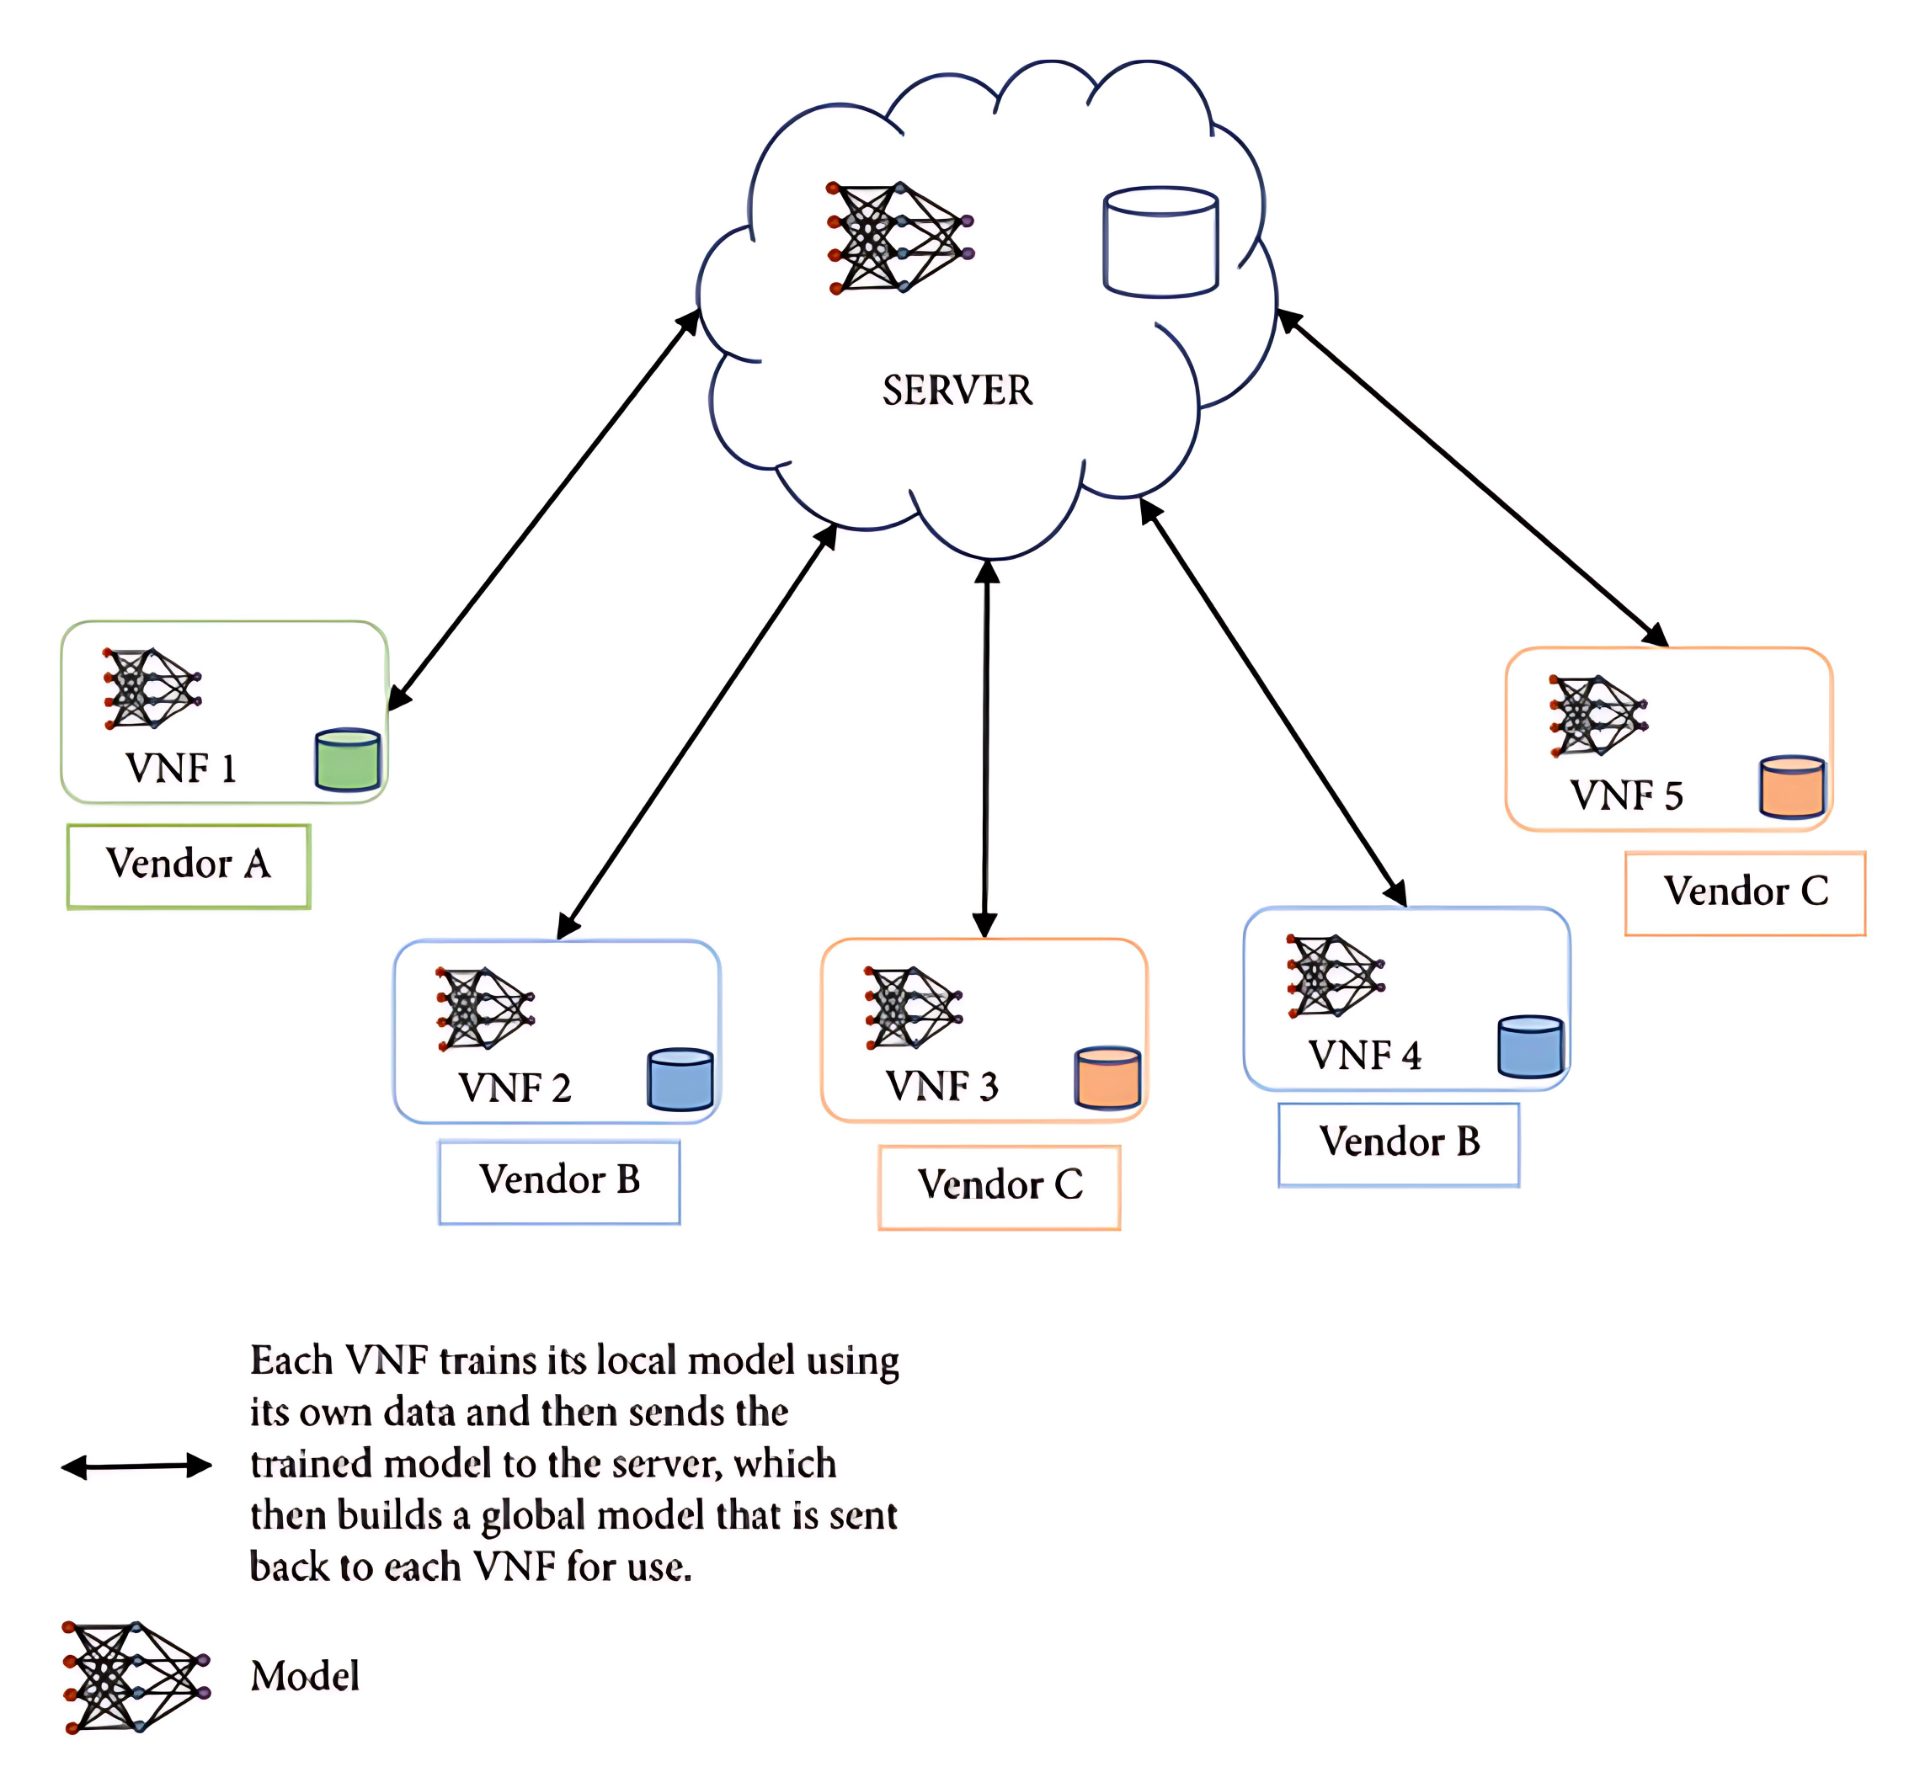
\includegraphics[width=0.85\textwidth]{./Figures/fig3.png}
    \caption{Figure 3 illustrates the architecture diversity across clients, showing how each local model (Virtual Network Function ) feeds into the broader federated learning system while maintaining autonomy over its training process.}
    \label{fig:local_models}
\end{figure}

\subsection{Stacking Ensemble Strategy}
\label{sec:stacking_ensemble_strategy}

Conventional federated learning (FL) methods like FedAvg assume that all clients use the same model architecture and share the same label space. However, this is rarely the case in real-world healthcare environments. To overcome these limitations, the proposed MStacking framework adopts a stacking ensemble strategy, which aggregates predictions instead of model parameters—making it flexible to both label and architectural heterogeneity.

The ensemble works in two levels (see Figure~\ref{fig:stacking_strategy}):

\begin{itemize}
    \item \textbf{Level-0 (Base Learners)}: Each client trains a binary classifier—such as a Random Forest (RF), Feedforward Neural Network (FNN), or Convolutional Neural Network (CNN)—on its local dataset. These models output probabilistic predictions for the normal class and one abnormal class.
    
    \item \textbf{Level-1 (Meta-Learner)}: A central model on the server aggregates predictions and density estimates (from Gaussian Mixture Models) sent by each client. It learns how to combine these varied outputs into a global multi-class classifier.
\end{itemize}

To enhance the quality of aggregation, each client also estimates the probability distribution of its input features and flags the classes it can recognize. These values are used to compute ensemble weights, which determine how much each client contributes to the final model.

As shown in Figure~\ref{fig:stacking_strategy}, this two-level stacking framework enables robust, privacy-preserving learning—even when clients have partial data or different computational capabilities.

\begin{figure}[h]
    \centering
    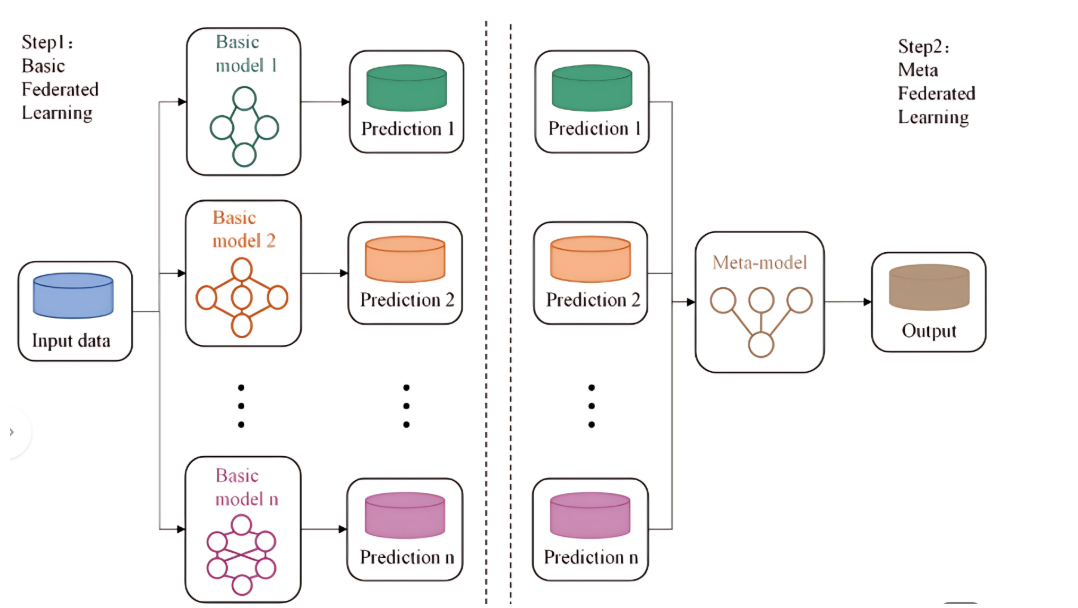
\includegraphics[width=0.85\textwidth]{./Figures/fig4.png}
    \caption{MStacking Two-Level Ensemble Architecture: Client-level models generate predictions and densities, aggregated by a central meta-learner into a global classifier.}
    \label{fig:stacking_strategy}
\end{figure}

\subsection{Federated Aggregation Process}
\label{sec:federated_aggregation}

Unlike traditional FL methods like FedAvg that rely on aggregating model parameters from identical architectures, MStacking takes a different route. It performs meta-level fusion, where predictions and feature distributions from each client’s model are combined at the server level.

Each participating client sends the following metadata to the central server:
\begin{itemize}
    \item Prediction probabilities from its trained binary classifier (e.g., RF, FNN, CNN).
    \item Density estimates of its local input data, modeled using Gaussian Mixture Models (GMMs).
    \item Class availability indicators that specify which classes the client has in its local dataset.
\end{itemize}

Using this information, the server constructs a global multi-class classifier $c_m(\theta)$ through a weighted integration of the client models. The weight $\omega_{j,m}$ assigned to client $j$ for class $m$ depends on:
\begin{itemize}
    \item Whether the class $m$ is present in client $j$’s data.
    \item The estimated quality of the local model, which factors in data distribution $f_{x_j}$ and the proportion of training samples from that client.
\end{itemize}

This aggregation strategy enables:
\begin{itemize}
    \item \textbf{Missing label handling}: Clients that lack some class labels can still contribute to the global model through inferred relationships.
    \item \textbf{Model flexibility}: Clients can use any architecture; uniformity is not required.
    \item \textbf{Privacy preservation}: Only high-level summaries (e.g., predictions and densities) are shared—never raw data or internal parameters.
\end{itemize}

\subsection{Evaluation Strategy}
\label{sec:evaluation_strategy}

To assess the performance and applicability of the MStacking framework, a structured evaluation plan will be followed using real-world and simulated data.

\textbf{Datasets:}
\begin{itemize}
    \item \textit{PhysioNet/CinC Challenge 2016}~\cite{clifford2016classification}: A large, annotated dataset of heart sounds, covering both normal and abnormal cases.
    \item \textit{Additional open-access PCG datasets}~\cite{liu2016open}: Used to simulate client-specific data distributions and class imbalances.
\end{itemize}

\textbf{Simulation Setup:}
\begin{itemize}
    \item Experiments will use Flower or FedML to simulate a federated environment.
    \item Clients will receive non-IID partitions, each containing the normal class and one abnormal class to replicate real-world heterogeneity.
\end{itemize}

\textbf{Metrics for Evaluation:}
\begin{itemize}
    \item Accuracy, Precision, Recall, F1-score (macro \& class-wise)
    \item AUROC for threshold robustness
    \item Confusion matrices to analyze prediction patterns
    \item Training time and communication cost for efficiency
    \item SHAP or similar methods for interpretability (if feasible)
\end{itemize}

\textbf{Baselines for Comparison:}
\begin{itemize}
    \item Centralized CNN trained on full data
    \item Traditional FedAvg with homogeneous models and labels
    \item Personalized FL with clustering or fine-tuning
\end{itemize}

\subsection{Implementation Details}
\label{sec:implementation}

\textbf{Development Environment:}
\begin{itemize}
    \item \textit{Language}: Python 3.x
    \item \textit{Federated Simulation}: Flower or FedML
    \item \textit{Deep Learning}: PyTorch
    \item \textit{Signal Processing}: OpenSMILE, LibROSA, and Continuous Wavelet Transform (CWT)
\end{itemize}

\textbf{Model Training:}
\begin{itemize}
    \item \textit{Optimizer}: Adam
    \item \textit{Monitoring}: Early stopping and validation tracking
    \item \textit{Architectures}: RF, FNN, CNN—based on local data modalities
\end{itemize}

\textbf{Execution Platform:}
\begin{itemize}
    \item \textit{Hardware}: Lab PCs or cloud-based GPUs (e.g., Google Colab, Kaggle)
    \item \textit{Version Control}: Git and GitHub
    \item \textit{Visualization \& Reporting}: Matplotlib, Seaborn, and LaTeX (Overleaf)
\end{itemize}

This implementation plan ensures that MStacking remains reproducible, scalable, and practical within an academic setting.
